\documentclass[11pt,a4paper,twoside]{report}

\author{Your Name}
\title{Thesis title}
\date{}

%\ProvidesPackage{jbd17style}

\usepackage[utf8x]{inputenc}
\usepackage[T1]{fontenc}
\usepackage{lmodern}
\usepackage{microtype}
\usepackage{ucs}
\usepackage{amsmath}
\usepackage{bm}
\usepackage{amsfonts}
\usepackage{textcomp}
\usepackage{amssymb}
\usepackage{graphicx}
\usepackage{wrapfig}
\usepackage{lipsum}
\usepackage[hidelinks, pdfa]{hyperref}
\usepackage{indentfirst}
\usepackage{siunitx}
\sisetup{separate-uncertainty}
\usepackage{chemformula}
\usepackage{hhline}
\usepackage{blindtext}
\usepackage{scontents}
\usepackage{titlesec}
\usepackage{tocbibind}
\usepackage{listings}
\usepackage{enumitem}

\usepackage{setspace}
\linespread{1.5}

\renewcommand{\thefootnote}{\fnsymbol{footnote}}

\usepackage[]{xcolor}
\definecolor{blue}{RGB}{13,71,161}
\definecolor{dark}{RGB}{0,60,112}
\definecolor{darker}{RGB}{0,40,74}
\definecolor{blackish}{RGB}{50,50,50}
\colorlet{defaultcolor}{.}
% Also tested 0 30 55, which was a bit too bright

\usepackage[export]{adjustbox}
\usepackage[margin={0cm,0.4cm}, oneside, indention=.4cm, labelfont={sc,color=darker}, textfont={small,color=blackish}]{caption}

\usepackage[superscript, nomove]{cite}
\makeatletter
\renewcommand{\@citess}[1]{\textsuperscript{[#1]}}
\makeatother

\newcommand{\citein}[1]{[\citen{#1}]}

\usepackage[left=2.5cm, right=2.5cm, top=2.5cm, bottom=2.5cm, includehead, nomarginpar]{geometry}

\usepackage{fancyhdr}
\pagestyle{fancy}
\fancyfoot{}
\cfoot{\color{dark}\rule[3.5pt]{1em}{0.5pt}~~\color{darker}\thepage~~\color{dark}\rule[3.5pt]{1em}{0.5pt}}
\fancyhead{}
\fancyhead[OR]{\color{darker}\rightmark}
\fancyhead[EL]{\color{darker}\leftmark}
\renewcommand{\headrulewidth}{0.5pt}
\renewcommand\headrule{%
	\nointerlineskip
	\smash{\color{dark}\rule{\headwidth}{\headrulewidth}}%
}
%\setlength{\headheight}{14pt}

\fancypagestyle{plain}{%
	\fancyhf{}%
	\fancyfoot[C]{\color{dark}\rule[3.5pt]{1em}{0.5pt}~~\color{darker}\thepage~~\color{dark}\rule[3.5pt]{1em}{0.5pt}}
	\renewcommand{\headrulewidth}{0pt}
}

\fancypagestyle{plainheadline}{%
	\fancyhf{}%
%	\fancyhead[C]{~}
	\renewcommand{\headrulewidth}{0pt}
	\fancyfoot[C]{\color{dark}\rule[3.5pt]{1em}{0.5pt}~~\color{darker}\thepage~~\color{dark}\rule[3.5pt]{1em}{0.5pt}}
}

% Adjust spacing in the list of figures to account for double-digit figure numbers
% https://tex.stackexchange.com/a/87027
% https://latexref.xyz/_005c_0040dottedtocline.html
\makeatletter
\renewcommand*\l@figure{\@dottedtocline{1}{1em}{2.9em}}
\makeatother

\makeatletter
\hypersetup{
	colorlinks=true,
	linkcolor=dark,
	citecolor=dark,
	urlcolor=dark,
	pdftitle=\@title
}
\makeatother
\usepackage{sectsty}
\sectionfont{\color{darker}}
\subsectionfont{\color{darker}}
\subsubsectionfont{\color{darker}}

\usepackage{chemformula}

\makeatletter
\let\c@table\c@figure % for (1)
\let\ftype@table\ftype@figure % for (2)
\makeatother

\usepackage{acronym}
% Very hacky way to make acronyms not blue...
%\makeatletter
%\renewcommand*{\ac}[2]{\hypersetup{linkcolor=.}\AC@starredfalse\protect\@ac{#1}{#2}\hypersetup{linkcolor=.}}
%%\WithSuffix\renewcommand\ac*{\AC@starredtrue\protect\@ac}
%\makeatother
%\renewcommand*\acsfont{\hypersetup{linkcolor=.}}
\renewcommand*\acffont{\emph}
\renewcommand*\acfsfont{\emph}

% .svg integration
\graphicspath{{figures/}}
\newcommand{\executeiffilenewer}[3]{
	\IfFileExists{#2}{}{
		\immediate\write18{#3}
	}
	\ifnum\pdfstrcmp{\pdffilemoddate{#1}}{\pdffilemoddate{#2}}>0{
		\immediate\write18{#3}
	}\fi%
}
\newcommand{\includesvg}[1]{%
	\executeiffilenewer{img/#1.svg}{img/exports/#1.pdf}%
	{inkscape -C --export-latex %
		--export-filename=img/exports/#1.pdf img/#1.svg}%
	\input{img/exports/#1.pdf_tex}%
}

\newcommand{\goodtilde}{{\raise.17ex\hbox{$\scriptstyle\mathtt{\sim}$}}}
\DeclareSIUnit\pulse{\text{pulse}}
\DeclareSIUnit\perpulse{\text{/pulse}}
%\DeclareSIUnit\fluence{\text{/pulse}}
\DeclareSIUnit\fluence{\micro\joule\per\centi\meter\squared\per\pulse}

\newenvironment{outline}{\begin{itemize}\color{blue}}{\end{itemize}}
\newenvsc{outlineDone}[store-env=forshort,print-env=false]
%\newenvironment{outline}
%	{\begin{outlineStore}\begin{itemize}\color{blue}}
%	{\end{itemize}\end{outlineStore}}
%\NewDocumentEnvironment{outline}{+b}{\begin{outlineStore}\begin{itemize}\color{blue}#1\end{itemize}\end{outlineStore}}{}

\newenvironment{originality}{\vspace{-2.7em}\small}{
	\par
	\color{dark}
	\noindent\rule{\textwidth}{0.5pt}
	\vspace{-.7em}
}

% Chapter format
\titleformat
{\chapter} % command
[display] % shape
{\centering\LARGE\color{darker}\bfseries\linespread{1}} % format
{
	\vspace{-6.05em}
	\rule{\textwidth}{0.pt}
	%\vspace{-0.6em}
	%\includegraphics[width=1.5in]{_headers/\thechapter.pdf}\\
	\chaptername~\thechapter
} % label
{0.5ex} % sep
{
	\Huge
} % before-code
[
	\vspace{-0.2em}
	\color{dark}
	\rule{\textwidth}{0.5pt}
] % after-code

\usepackage{epigraph}
\setlength{\epigraphwidth}{0.8\textwidth}
\renewcommand{\textflush}{flushepinormal}
\setlength{\beforeepigraphskip}{-\baselineskip}
\setlength{\afterepigraphskip}{2\baselineskip}
\setlength{\epigraphrule}{0.5pt}
\makeatletter
\renewcommand{\@epirule}{\color{dark}\rule[1ex]{\epigraphwidth}{\epigraphrule}}
\makeatother

% Little decorations
\usepackage{tikz}
\def\checkmark{
	\tikz\fill[scale=0.5](0,.55) -- (.25,0.2) -- (1,.9) -- (.25,.35) -- cycle;
}
\def\notion{
	\def \globalscale {.17}
	\begin{tikzpicture}[yscale=\globalscale,xscale=\globalscale, every node/.append style={scale=\globalscale}, inner sep=0pt, outer sep=0pt, baseline=0.9pt]
		\path[fill,even odd rule] (1.6232, 2.6398) -- (0.1592, 2.5317).. controls (0.0411, 2.5215) and (0.0, 2.4443) .. (0.0, 2.3518) -- (0.0, 0.7468).. controls (0.0, 0.6748) and (0.0256, 0.6131) .. (0.0873, 0.5308) -- (0.4315, 0.0833).. controls (0.488, 0.0112) and (0.5394, -0.0042) .. (0.6474, 0.0009) -- (2.3475, 0.1038).. controls (2.4912, 0.1141) and (2.5324, 0.181) .. (2.5324, 0.2941) -- (2.5324, 2.0997).. controls (2.5324, 2.1582) and (2.5093, 2.1751) .. (2.4413, 2.225) -- (1.9623, 2.5627).. controls (1.8493, 2.6449) and (1.8031, 2.6553) .. (1.6232, 2.6399) -- cycle(0.6858, 2.1293).. controls (0.547, 2.1199) and (0.5155, 2.1178) .. (0.4366, 2.1819) -- (0.2362, 2.3414).. controls (0.2158, 2.362) and (0.2261, 2.3878) .. (0.2774, 2.3929) -- (1.6848, 2.4957).. controls (1.803, 2.5061) and (1.8645, 2.4649) .. (1.9107, 2.4289) -- (2.1521, 2.254).. controls (2.1624, 2.2488) and (2.1881, 2.218) .. (2.1572, 2.218) -- (0.7038, 2.1305) -- (0.6858, 2.1293) -- cycle(0.524, 0.3096) -- (0.524, 1.8424).. controls (0.524, 1.9093) and (0.5445, 1.9402) .. (0.6061, 1.9454) -- (2.2754, 2.0431).. controls (2.332, 2.0482) and (2.3576, 2.0122) .. (2.3576, 1.9454) -- (2.3576, 0.4228).. controls (2.3576, 0.3559) and (2.3473, 0.2992) .. (2.2549, 0.2941) -- (0.6574, 0.2015).. controls (0.565, 0.1964) and (0.524, 0.2272) .. (0.524, 0.3096) -- cycle;
		\path[fill,even odd rule] (2.1009, 1.7602).. controls (2.1111, 1.7139) and (2.1009, 1.6676) .. (2.0546, 1.6623) -- (1.9776, 1.647) -- (1.9776, 0.5153).. controls (1.9107, 0.4793) and (1.8492, 0.4588) .. (1.7977, 0.4588).. controls (1.7155, 0.4588) and (1.695, 0.4845) .. (1.6334, 0.5616) -- (1.1299, 1.3538) -- (1.1299, 0.5874) -- (1.2892, 0.5513).. controls (1.2892, 0.5513) and (1.2892, 0.4587) .. (1.1607, 0.4587) -- (0.8064, 0.4381).. controls (0.7961, 0.4588) and (0.8064, 0.5102) .. (0.8423, 0.5204) -- (0.9349, 0.5461) -- (0.9349, 1.5595) -- (0.8065, 1.5699).. controls (0.7961, 1.6162) and (0.8218, 1.683) .. (0.8938, 1.6882) -- (1.2739, 1.7138) -- (1.7978, 0.9114) -- (1.7978, 1.6213) -- (1.6642, 1.6366).. controls (1.6539, 1.6933) and (1.695, 1.7345) .. (1.7463, 1.7395) -- (2.1009, 1.7602) -- cycle;
	\end{tikzpicture}
}
\def\paper{
	\def \globalscale {.17}
	\begin{tikzpicture}[yscale=\globalscale,xscale=\globalscale, every node/.append style={scale=\globalscale}, inner sep=0pt, outer sep=0pt, baseline=0.9pt]
		\path[draw,line cap=round,line join=round,line width=0.043cm] (0.4291, 2.5743) -- (1.5339, 2.5743) -- (2.2168, 1.8914) -- (2.2168, 0.0715) -- (0.4291, 0.0715) -- cycle;
		\path[draw,line cap=round,line join=round,line width=0.043cm] (1.5339, 2.5743) -- (1.5339, 1.8914) -- (2.2168, 1.8914);
	\end{tikzpicture}
}
\def\globe{
	\def \globalscale {.17}
	\begin{tikzpicture}[yscale=\globalscale,xscale=\globalscale, every node/.append style={scale=\globalscale}, inner sep=0pt, outer sep=0pt, baseline=0.9pt]
		\path[draw,line cap=round,line join=round,line width=0.023cm] (0.0768, 1.3229) -- (2.569, 1.3229);
		\path[draw,line join=round,line width=0.023cm] (2.569, 1.3229)arc(0.0:90.0:1.2461 and -1.2461)arc(90.0:180.0:1.2461 and -1.2461)arc(180.0:270.0:1.2461 and -1.2461)arc(-90.0:0.0:1.2461 and -1.2461) -- cycle;
		\path[draw,line cap=round,line join=round,line width=0.023cm] (1.3229, 2.569) -- (1.3229, 0.0768);
		\path[draw,line cap=round,line join=round,line width=0.023cm] (1.3229, 2.569).. controls (2.3544, 2.022) and (2.2875, 0.534) .. (1.3229, 0.0768);
		\path[draw,line cap=round,line join=round,line width=0.023cm] (1.3229, 2.569).. controls (0.2914, 2.022) and (0.3583, 0.534) .. (1.3229, 0.0768);
		\path[draw,line join=round,line width=0.023cm] (0.4058, 2.1665).. controls (1.0172, 1.9285) and (1.6286, 1.9285) .. (2.24, 2.1665);
		\path[draw,line join=round,line width=0.023cm] (0.4058, 0.4793).. controls (1.0172, 0.7173) and (1.6286, 0.7173) .. (2.24, 0.4793);
	\end{tikzpicture}
}
\def\progress{
	\def \globalscale {.17}
	\begin{tikzpicture}[yscale=\globalscale,xscale=\globalscale, every node/.append style={scale=\globalscale}, inner sep=0pt, outer sep=0pt, baseline=0.9pt]
		\path[draw,line join=round,line width=0.0524cm] (2.2318, 2.5475).. controls (2.2318, 1.9291) and (1.8249, 1.4277) .. (1.3229, 1.4277).. controls (0.821, 1.4277) and (0.414, 1.9291) .. (0.414, 2.5475) -- cycle;
		\path[draw,line join=round,line width=0.0524cm] (2.2318, 0.0768).. controls (2.2318, 0.6953) and (1.8249, 1.1966) .. (1.3229, 1.1966).. controls (0.821, 1.1966) and (0.414, 0.6953) .. (0.414, 0.0768) -- cycle;
		\path[fill,line join=round,line width=0.043cm] (1.1061, 1.4689) rectangle (1.5397, 1.1724);
		\path[fill,line join=round,line width=0.0768cm] (0.2803, 2.6458) rectangle (2.3656, 2.4492);
		\path[fill,line join=round,line width=0.0768cm] (0.2803, 0.1967) rectangle (2.3656, -0.0);
		\path[fill,line join=round,line width=0.0524cm] (2.1604, 2.1116).. controls (2.1144, 1.9777) and (2.0478, 1.857) .. (1.9656, 1.7557).. controls (1.8011, 1.5531) and (1.5739, 1.4277) .. (1.3229, 1.4277).. controls (1.0719, 1.4277) and (0.8447, 1.5531) .. (0.6802, 1.7557).. controls (0.598, 1.857) and (0.5315, 1.9777) .. (0.4855, 2.1116).. controls (0.4395, 2.2456) and (2.2064, 2.2456) .. (2.1604, 2.1116) -- cycle;
		\path[draw,line join=round,line width=0.043cm] (1.3229, 1.3229) -- (1.3229, 0.1967);
	\end{tikzpicture}
}

% If you only want to include specific sections to speed up compilation,
% specify a list here.
%\includeonly{sections/example}

\begin{document}

\begin{titlepage}
	% Make sure the title page appears in the Table of Contents (TOC)
	\addcontentsline{toc}{chapter}{Title page}
	\vspace*{-0.75in}
	\hspace*{-.25in}
	% I don't have the license to distribute the actual Imperial logo, please source it from https://brand.imperial.ac.uk/document/36/show/eyJpZCI6Mjg4LCJzY29wZSI6ImFzc2V0OnZpZXciLCJ0aW1lc3RhbXAiOiIxNzcyNDcwMjkxIn0:imperial-college-london:1tHxM2Zuwy9tzqAjfV-YTl6koKG5PeGPwZ67blkqy80 (aim for the CMYK blue logo in the .eps format, better for print) or replace with the appropiate logo for your university.
	%	\includegraphics[width=0.5\textwidth]{_headers/IMPERIAL_logo_CMYK_Blue_2024.eps}
	
\includegraphics[width=0.5\textwidth]{_headers/fake-Imperial-logo.pdf}
%	\begin{center}
		\vspace*{2cm}
		\makeatletter
		\begin{spacing}{1.3}
			\noindent\Huge\color{darker}\scshape\bfseries\@title
		\end{spacing}

		\vspace{-.3cm}
		\large
		\noindent A thesis submitted in partial fulfilment of the requirements for the PhD degree.

		\vspace{1.5cm}
		\noindent\textbf{\@author} \\
		\noindent Imperial College London\\
		Department of Physics\\
		June 2025

		\makeatother

		\vspace{3.cm}
		\large
		\noindent Supervision:

		\vspace{0.7cm}
		\noindent\textbf{Prof. One} \\
		\emph{Imperial College London}

		\vspace{0.7cm}
		\noindent\textbf{Prof. Two} \\
		\emph{Another University}

		\vspace{0.7cm}
		\noindent\textbf{Prof. Threee} \\
		\emph{A Third University}

		\vspace{1.5cm}

%	\end{center}
\end{titlepage}

% Inlcude the abstract, acknowledgments, etc
% This file contains your abstract, copyright statement, acknowledgments, and anything you want to appear at the start of the document.

% Section headers here should not be numbered...
\chapter*{Abstract}
% But that means they have to be added to the table of contents manually
\addcontentsline{toc}{chapter}{Abstract}
% 300 words at Imperial.
\lipsum[1-2]

\chapter*{Copyright and originality statements}
\addcontentsline{toc}{chapter}{Copyright and originality statements}
The copyright of this thesis rests with the author.
Unless otherwise indicated, its contents are licensed under a Creative Commons Attribution-Non Commercial 4.0 International Licence (CC BY-NC 4.0).

Under this licence, you may copy and redistribute the material in any medium or format.
You may also create and distribute modified versions of the work.
This is on the condition that you credit the author and do not use it, or any derivative works, for a commercial purpose.

When reusing or sharing this work, ensure you make the licence terms clear to others by naming the licence and linking to the licence text.
Where a work has been adapted, you should indicate that the work has been changed and describe those changes.

The text above is a summary and does not constitute the legally-binding license.
Please consult the complete text of the CC BY-NC 4.0 license at \url{https://creativecommons.org/licenses/by-nc/4.0/legalcode.en} for the full details of this agreement.

Please seek permission from the copyright holder for uses of this work that are not included in this licence or permitted under UK Copyright Law.

The work, text, and figures presented in this thesis are my own unless otherwise stated.
Where work from publications on which I am co-author is adapted, this is made clear in the heading of the corresponding chapter.

\chapter*{Acknowledgments}
\addcontentsline{toc}{chapter}{Acknowledgments}
% When a section extends beyond a single page, use \markboth to make the header title correct
\markboth{\scshape ACKNOWLEDGMENTS}{\scshape ACKNOWLEDGMENTS}

% Add a quote if you want!
\epigraph{Example quote}{\textit{Book title, \textsc{A. Uthor}}}

\lipsum[3-7]

\chapter*{List of publications}
\addcontentsline{toc}{chapter}{List of publications}

\subsection*{Major contributions}
\hyphenation{Stenning}
\begin{itemize}
	\item \textbf{J.~Dranczewski}, A.~Fischer, P.~Tiwari, M.~Scherrer, D.~Saxena, H.~Schmid, R.~Sapienza, K.~Moselund, ``\href{https://doi.org/10.1016/j.mne.2023.100196}{Plasma etching for fabrication of complex nanophotonic lasers from bonded InP semiconductor layers}'' \textit{Micro and Nano Engineering}, vol. 19, p. 100196, Jun. 2023.

	\item D.~Saxena,\footnotemark[1] A.~Fischer,\footnotemark[1] \textbf{J.~Dranczewski}, W.~K.~Ng, N.~V.~Trivino, H.~Schmid, T.~V.~Raziman, A.~Arnaudon, M.~Barahona, O.~Hess, K.~Moselund, R.~Sapienza, ``\href{https://doi.org/10.1002/lpor.202400623}{Designed Semiconductor Network Random Lasers},'' \textit{Laser \& Photonics Reviews}, vol. 19, no. 1, p. 2400623, 2024.

	\item \textbf{J.~Dranczewski},\footnotemark[1] W.~K.~Ng,\footnotemark[1] A.~Fischer,\footnotemark[1] T.~V.~Raziman, D.~Saxena, T.~Farchy, K.~Stenning, J.~Peters, H.~Schmid, W.~R.~Branford, M.~Barahona, K.~Moselund, R.~Sapienza, J.~C.~Gartside, ``\href{https://doi.org/10.48550/arXiv.2407.15558}{Retinomorphic Machine Vision in a Network Laser},'' \textit{arXiv}, Aug. 2025. \textit{[manuscript in review]}
\end{itemize}

\subsection*{Minor contributions}
\begin{itemize}
	\item A.~Fischer, T.~V.~Raziman, W.~K.~Ng, J.~Clarysse, D.~Saxena, \textbf{J.~Dranczewski}, S.~Vezzoli, H.~Schmid, K.~Moselund, R.~Sapienza, ``\href{https://doi.org/10.1038/s44310-024-00006-9}{Controlling lasing around exceptional points in coupled nanolasers},'' \textit{npj Nanophotonics}, vol. 1, no. 1, pp. 1–6, May 2024.
	\item A.~Fischer,\footnotemark[1] T.~Severs Millard,\footnotemark[1] X.~Xiao, T.~V.~Raziman, \textbf{J.~Dranczewski}, R.~C.~Schofield, H.~Schmid, K.~Moselund, R.~Sapienza, R.~F.~Oulton, ``\href{https://doi.org/10.1021/acsphotonics.4c01236}{Surface Lattice Resonance Lasers with
	Epitaxial InP Gain Medium},'' \textit{ACS Photonics}, vol. 11, no. 10, pp. 4316–4322, Oct. 2024.
\end{itemize}

\footnotetext[1]{Authors contributed equally.}


% Microtype should be disabled for the table of contents and similar,
% since it can mess up the alignment of the numbers
\microtypesetup{protrusion=false}

% TOC and figure list
\tableofcontents
\listoffigures

% Acronyms
\newpage
\chapter*{Acronyms}

% These are required to add an unnumbered section to the table of contents
% and display correct headers
\addcontentsline{toc}{chapter}{Acronyms}
\markboth{\scshape ACRONYMS}{\scshape ACRONYMS}

% Use https://ctan.org/pkg/acronym?lang=en to generate an acronym list.
% In the text, you would use:
% \ac{CPU} - the first instance of the acronym will be expanded, and all uses link back to the acronym list
% \acf{CPU} - print the expanded version of the acronym
% \Ac{CPU} or \Ac{CPU} - start the expanded version of the acronym with a capital letter.
% See the documentation linked above for details

\begin{acronym}[ABCDEFGH]
	\setlength\itemsep{.0em}
	\item \textbf{Computing}
	\acro {AI} {Artificial Intelligence}
	\acro {API} {Application Programming Interface}
	\acro {CNN} {Convolutional Neural Network}
	\acro {CPU} {Central Processing Unit}
	\acro {GPU} {graphics processing unit}
	\acro {GUI} {Graphical User Interface}
	\acro {LLM} {Large Language Model}
	\acro {ML} {Machine Learning}
	\acro {MLP} {multilayer perceptron}
	\acro {RAM} {Random Access Memory}
	\acro {RGB} {red, green, and blue}
	\vspace{1em}

	\item \textbf{Fabrication}
	\acro {ALD} {Atomic Layer Deposition}
	\acro {BOX} {burried oxide}
	\acro {DoE} {Design of Experiment}
	\acro {DWB} {Direct Wafer Bonding}
	\acro {FIB} {Focused Ion Beam}
	\acro {HSQ} {hydrogen silsesquioxane}
	\acro {ICP} {Inductively Coupled Plasma}
	\acro {MOCVD} {metalorganic chemical vapour deposition}
	\acro {PECVD} {plasma-enhanced chemical vapour deposition}
	\acro {QD} {quantum dot}
	\acro {QW} {quantum well}
	\acro {RF}  {Radio Frequency}
	\acro {RIE} {Reactive Ion Etching}
	\acro {TASE} {Template-Assisted Selective Epitaxy}
	\acro {VCSEL} {Vertical Cavity Surface Emitting Laser}
	\vspace{1em}

\end{acronym}

% back to normal microtype settings for the rest of the text
\microtypesetup{protrusion=true}

%%%%%%%%%%%%%%%%%%%%%%%%%%%%%%%

% Include all your sections here
\chapter{Example chapter}
% Give your sections labels so you can refer to them from other spots (this works across .tex files in the "sections" folder too!).
\label{ch:example}

% Include a statement of originality describing your contributions at the start of the chapter
\begin{originality}
	For the work presented in this chapter I have contributed <X>.
	Most figures in this section, as well as parts of the relevant discussion, are adapted from the following publication, plotting for which has been done by me, and a couple of other people:

	J.~Dranczewski,\footnotemark[1] W.~K.~Ng,\footnotemark[1] A.~Fischer,\footnotemark[1] T.~V.~Raziman, D.~Saxena, T.~Farchy, K.~Stenning, J.~Peters, H.~Schmid, W.~R.~Branford, M.~Barahona, K.~Moselund, R.~Sapienza, J.~C.~Gartside, ``\href{https://doi.org/10.48550/arXiv.2407.15558}{Retinomorphic Machine Vision in a Network Laser},'' \textit{arXiv}, Aug. 2024. \textit{[manuscript in review]}
\end{originality}

%\footnotetext[1]{Authors contributed equally.}
% Use a custom text instead of the default footnote, which would go to the bottom of the page.
\vspace{-1.5em}
{\footnotesize*Authors contributed equally.}

\section*{Abstract}
% Include a brief chapter abstract if desired.
The header images are optional, and described in more detail in `thesis\_style.sty'. Basically, put a .pdf file matching the chapter number/letter in `figures/\_headers`, and you'll get a chapter header image. If there's no file for a chapter, it defaults to `default.pdf`. Remove that file -- no headers!

\lipsum[1]

\section{Example section}
\label{sec:example_section}
\begin{outline}
	\item You can write notes to yourself in ``outline'' environments. They act like LaTeX's ``itemize'', but are coloured blue, and you can easily hide them from the final document once you're done with a specific outline by changing the environment name to ``outlineDone''.
	\item I also provide a number of potentially useful icons that can be used to annotate these outlines:
	\begin{itemize}
		\item Checkmarks, for points you've covered \checkmark
		\item Hourglass for things that are in progress \progress
		\item Paper, for things to be adapted from papers \paper
		\item Globe, for things that need to be referenced or researched from external sources \globe
		\item Notion, as that's where I was tracking figure progress \notion
	\end{itemize}
	\item You can use these anywhere in the text just by using the commands listed in the source above: \checkmark\paper
\end{outline}

\begin{outlineDone}
	\item This outline will not appear in the compiled document, but you can keep it in the source for reference.
\end{outlineDone}

Example citation\cite{dranczewskiPlasmaEtchingFabrication2023} -- citations appear in the upper right by default, if you need to reference a citation in the main text you can use Ref.~\citein{dranczewskiPlasmaEtchingFabrication2023}. Note the \goodtilde~symbol -- it forms a non-breaking space between ``Ref.'' and the citation number, meaning that they will always appear on the same line. You can similarly reference chapters and sections, for example Chapter~\ref{ch:example}.

Here's an example figure: Fig.~\ref{fig:z_example_a_name}

\begin{figure}[h]
	\centering
	% You'll note that I'm not including a figure width here - in my opinion you should prepare the figures
	% to be the correct width from the start, which avoids any rescaling issues or font size discrepancies.
	% For this document, the figure width should be 6.3 inches
	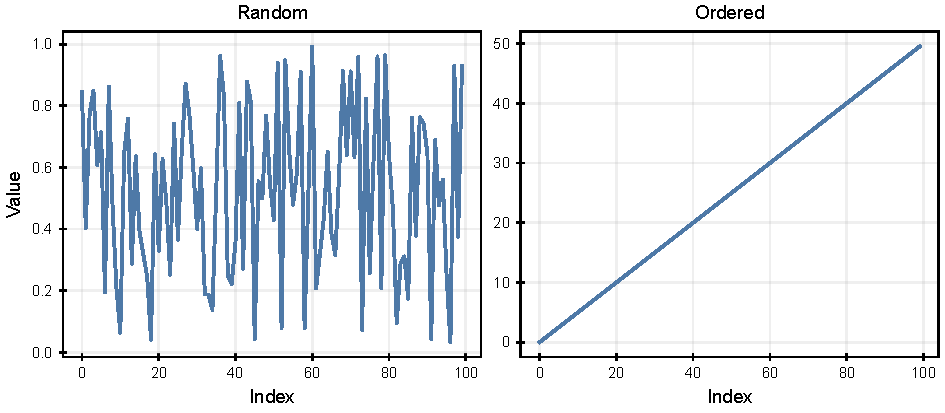
\includegraphics{z_example_a_name/z_example_a_name.pdf}
	\caption[
		Wide example figure % This short description will appear in the figure list
	]{
		% This long description will appear in the text.
		Example figure description.
		\textbf{a}~This describes part \textit{a} of the figure.
		\textbf{b}~This describes part \textit{b} of the figure.
	}
	% Provide an ID for the figure so it can be referenced elsewhere in the text.
	% Mine follow a scheme of [sequential chapter letter]_[short chapter name]_[sequential figure letter]_[short figure name]
	% This allows easy alphabetical sorting of the figure folders, and general consistency.
	\label{fig:z_example_a_name}
\end{figure}

Here's an example of a narrow figure with the caption to the side: Fig.~\ref{fig:a_example_b_narrow}. You can use `figures/placeholder.pdf' as temporary content while you work on the real figures.

% Here we make the figure narrower, add some horizontal fill, and then add the caption to the right in a "minipage"
\begin{figure}[h]
	% If you do need to specify a figure width, this is how.
	
\includegraphics[width=2.2in, valign=c]{placeholder.pdf}
	\hfill
	\begin{minipage}{\dimexpr \textwidth-\columnsep-2.2in}
		\captionsetup{skip=0pt}
		\caption[
			Narrow example figure
		]{
			Narrow figure caption.
		}
		\label{fig:a_example_b_narrow}
	\end{minipage}
\end{figure}

Examples of acronym usage: first instance -- \ac{CPU}, second instance -- \ac{CPU}. Forced full: \acf{CPU}.
Examples of `siunitx' usage: \qty{1.23}{\meter\squared}, \qty{45.6}{\fluence} (custom unit defined in `thesis\_style.tex').
Chemical formula: \ch{Al2(SO4)3}

%%%%%%%%%%%%%%%%%%%%%%%%%%%%%%%

% Appendix time!
\appendix
% Make the chapter headers say "Appendix" instead of "Chapter"
\renewcommand{\chaptername}{Appendix}
\chapter{Example appendix}
% If your chapter doesn't have sections (which are normally marked in the right corner),
% manually tell LaTeX to put the chapter name in there.
\markright{\scshape\uppercase{Example appendix}}

\lipsum[1-3]

\chapter*{Reproduction permissions}
\markright{\scshape\uppercase{Reproduction permissions}}
% Need to add unnumbered chapters to the table of contents manually
\addcontentsline{toc}{chapter}{Reproduction permissions}
When necessary, the appropriate license and a link to its full text have been provided directly next to any reproduced figures, or in the originality statement in the chapter heading. For print copies of the thesis, the links to the relevant licenses are reproduced verbatim here:
\begin{itemize}
	\item CC BY 4.0 -- \url{https://creativecommons.org/licenses/by/4.0/}
	\item CC BY-NC 4.0 -- \url{https://creativecommons.org/licenses/by-nc/4.0/}
\end{itemize}

\vspace{4ex}
The LaTeX template used to prepare this thesis was created by J. Dranczewski and is available at \url{https://github.com/jdranczewski/phd-thesis-template}.

\vspace{4ex}
Here's an example of pasting in a full license text:

\begin{lstlisting}[basicstyle=\footnotesize, upquote=false]
MIT License

Copyright (c) 2026 <name>

Permission is hereby granted, free of charge, to any person obtaining a copy
of this software and associated documentation files (the "Software"), to deal
in the Software without restriction, including without limitation the rights
to use, copy, modify, merge, publish, distribute, sublicense, and/or sell
copies of the Software, and to permit persons to whom the Software is
furnished to do so, subject to the following conditions:

The above copyright notice and this permission notice shall be included in all
copies or substantial portions of the Software.

THE SOFTWARE IS PROVIDED "AS IS", WITHOUT WARRANTY OF ANY KIND, EXPRESS OR
IMPLIED, INCLUDING BUT NOT LIMITED TO THE WARRANTIES OF MERCHANTABILITY,
FITNESS FOR A PARTICULAR PURPOSE AND NONINFRINGEMENT. IN NO EVENT SHALL THE
AUTHORS OR COPYRIGHT HOLDERS BE LIABLE FOR ANY CLAIM, DAMAGES OR OTHER
LIABILITY, WHETHER IN AN ACTION OF CONTRACT, TORT OR OTHERWISE, ARISING FROM,
OUT OF OR IN CONNECTION WITH THE SOFTWARE OR THE USE OR OTHER DEALINGS IN THE
SOFTWARE.
\end{lstlisting}

\bibliographystyle{myIEEEtran}
% we're making the bibliography take a little less space here
\begin{spacing}{1.25}
	\small
	% argument is your BibTeX string definitions and bibliography database(s)
	% export "library.bib" from Zotero, I recommend looking up BetterBibTeX
	\bibliography{IEEEabrv,library.bib}
\end{spacing}

\end{document}
